\chapter{Visualizing Large Models}
\label{chap:VisualizingLargeModels}

\begin{inlinefig}
  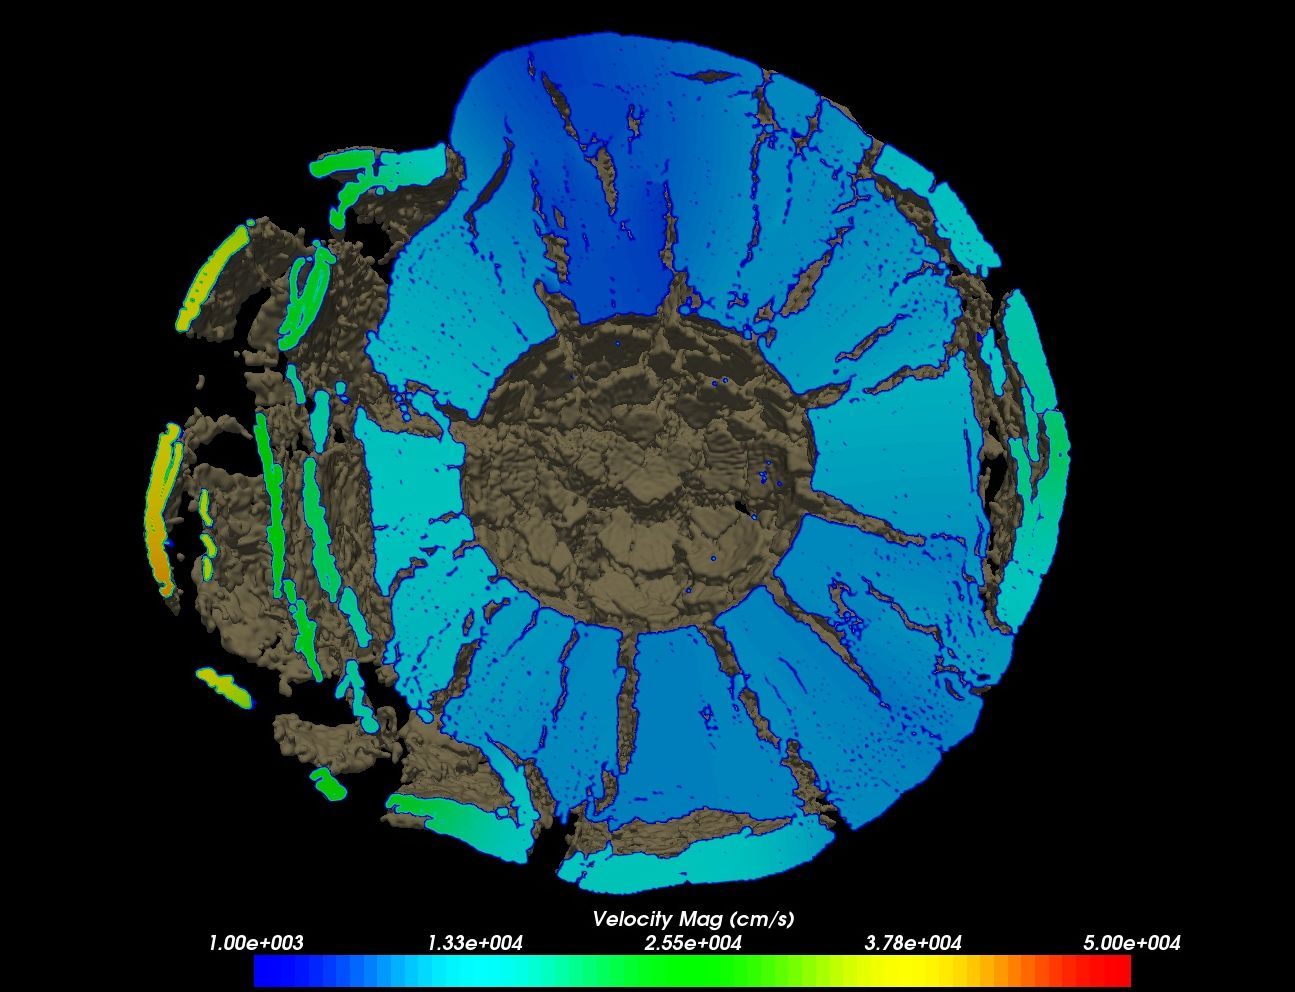
\includegraphics[height=1.8in]{images/Asteroid}
  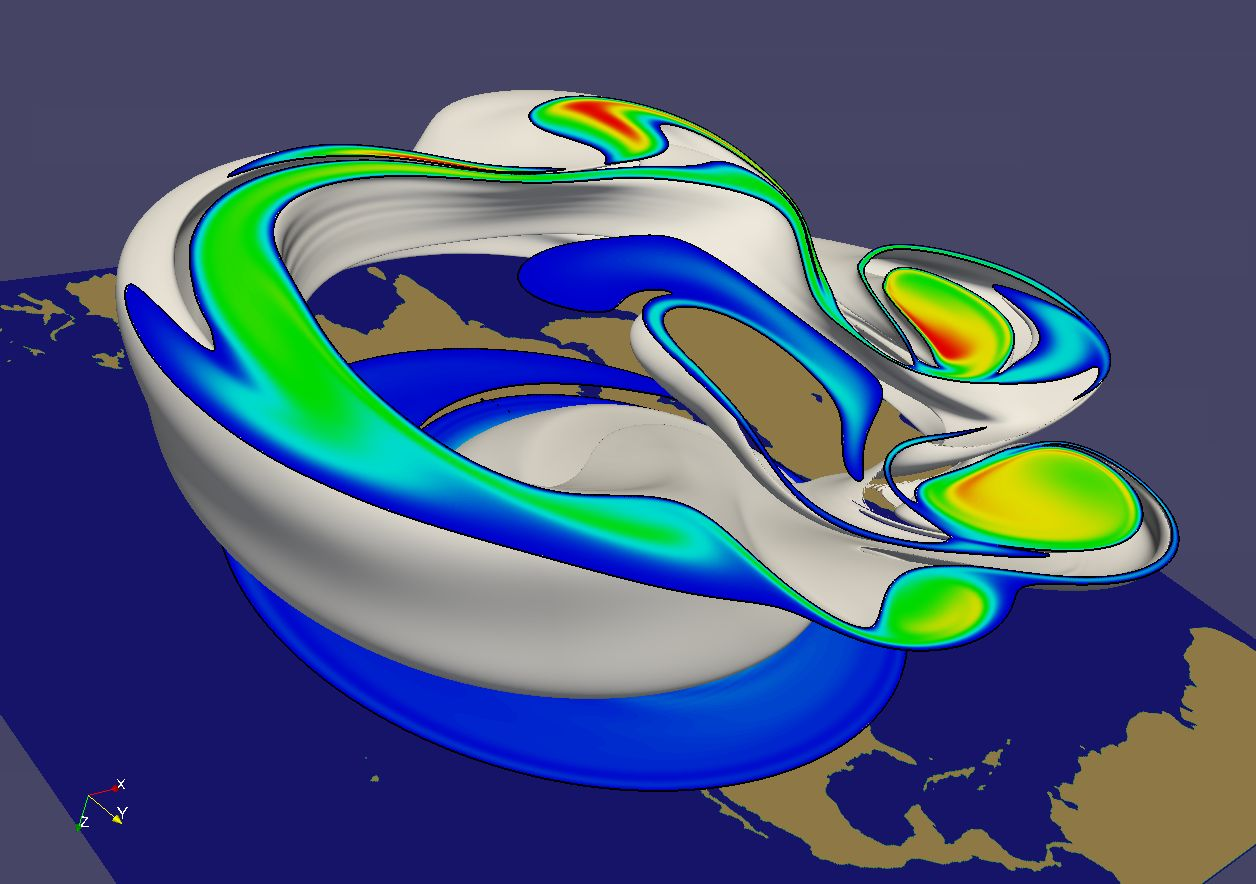
\includegraphics[height=1.8in]{images/PolarVortex} \\ \vspace{.5ex}
  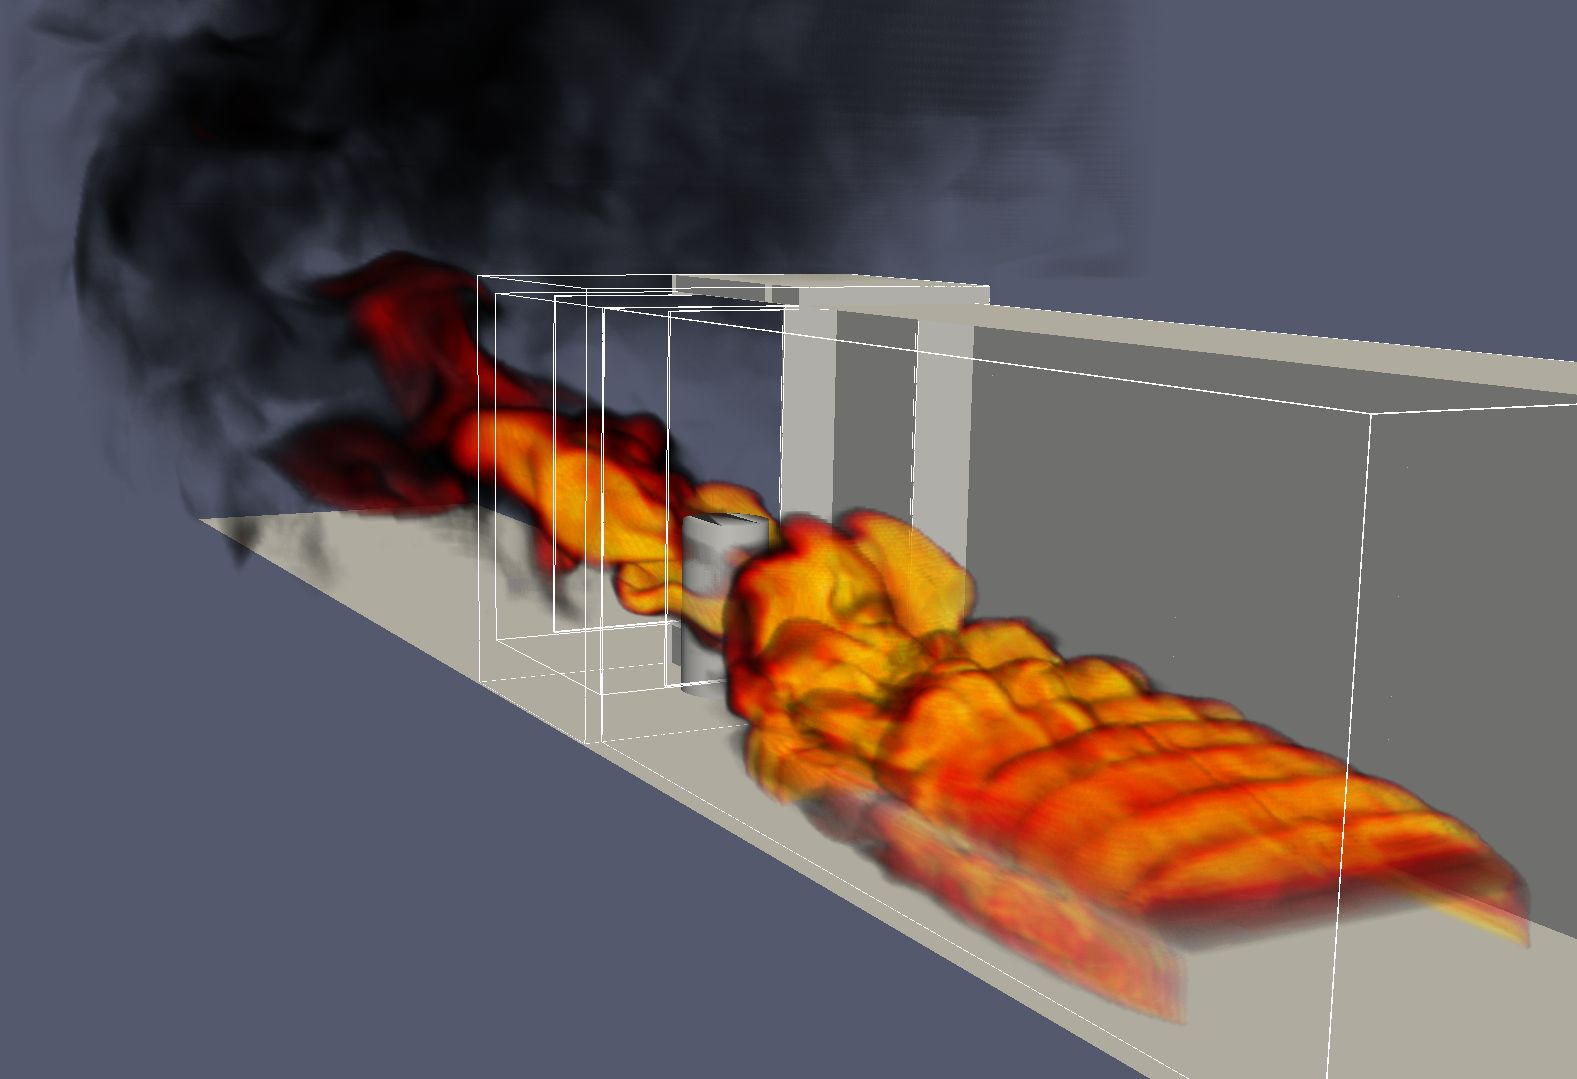
\includegraphics[height=1.8in]{images/Fire}
  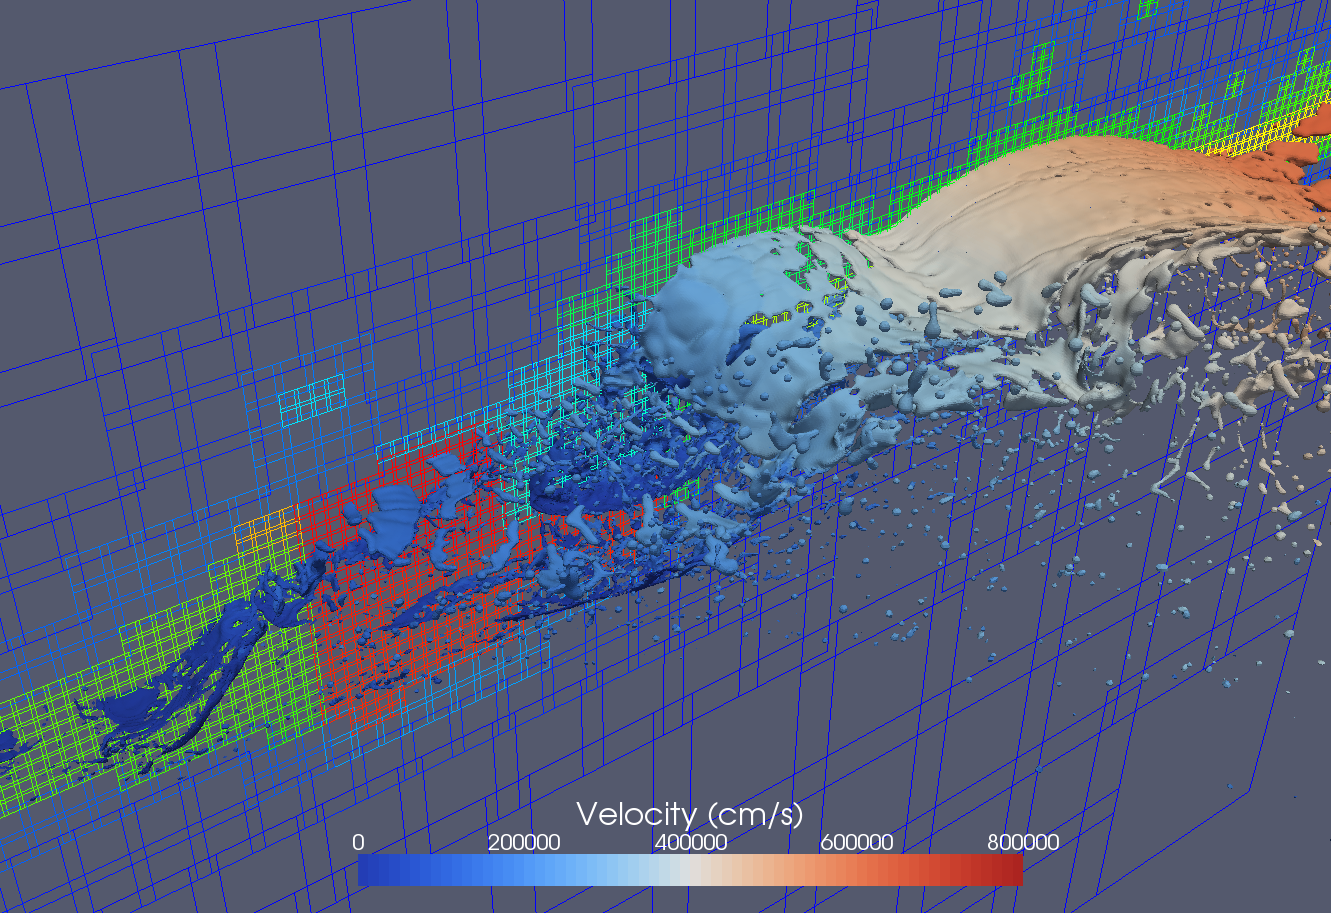
\includegraphics[height=1.8in]{images/LargeAMR}
\end{inlinefig}

ParaView is used frequently at Sandia National Laboratories for visualizing
data from large-scale simulations run on the Red Storm supercomputer such
as the examples shown here.  The upper left image shows a CTH shock physics
simulation with over 1 billion cells of a 10 megaton explosion detonated at
the center of the Golevka asteroid.  The upper right image shows a SEAM
Climate Modeling simulation with 1 billion cells modeling the breakdown of
the polar vortex, a circumpolar jet that traps polar air at high latitudes.
The lower left image shows a loosely coupled SIERRA/Fuego/Syrinx/Calore
simulation with 10 million unstructured hexahedra cells of
objects-in-crosswind fire.  The lower right image shows a CTH simulation
that generates AMR data.  We have used ParaView to visualize CTH simulation
AMR data comprising billions of cells, 100’s of thousands of blocks, and
eleven levels of hierarchy (not shown).

In this section we discuss visualizing large meshes like these using the
parallel visualization capabilities of ParaView.  This section is less
“hands-on” than the previous section.  You will learn the conceptual
knowledge needed to perform large parallel visualization instead.  We
present the basic ParaView architecture and parallel algorithms and
demonstrate how to apply this knowledge.


\section{ParaView Architecture}

ParaView is designed as a three-tier client-server architecture.  The three
logical units of ParaView are as follows.

\begin{description}
\item[Data Server] \index{data server} The unit responsible for data
  reading, filtering, and writing.  All of the pipeline objects seen in the
  pipeline browser are contained in the data server.  The data server can
  be parallel.
\item[Render Server] \index{render server}The unit responsible for
  rendering.  The render server can also be parallel, in which case built
  in parallel rendering is also enabled.
\item[Client] \index{client}The unit responsible for establishing
  visualization.  The client controls the object creation, execution, and
  destruction in the servers, but does not contain any of the data (thus
  allowing the servers to scale without bottlenecking on the client).  If
  there is a GUI, that is also in the client.  The client is always a
  serial application.
\end{description}

These logical units need not by physically separated.  Logical units are
often embedded in the same application, removing the need for any
communication between them.  There are three modes in which you can run
ParaView.

\begin{inlinefig}
  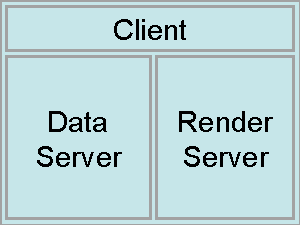
\includegraphics{images/RunModeStandalone}
\end{inlinefig}

The first mode, which you are already familiar with, is
\keyterm{standalone} mode.  In standalone mode, the client, data server,
and render server are all combined into a single serial application.  When
you run the \commandline{paraview} application, you are automatically connected
to a \keyterm{builtin} server so that you are ready to use the full
features of ParaView.

\begin{inlinefig}
  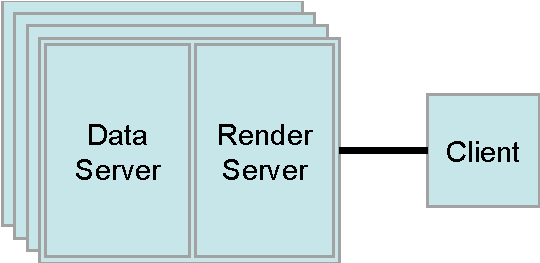
\includegraphics{images/RunModeClientServer}
\end{inlinefig}

The second mode is \keyterm{client-server} mode.  In client-server mode,
you execute the \commandline{pvserver} program on a parallel machine and
connect to it with the \commandline{paraview} client application.  The
\commandline{pvserver} program has both the data server and render server
embedded in it, so both data processing and rendering take place there.
The client and server are connected via a socket, which is assumed to be a
relatively slow mode of communication, so data transfer over this socket is
minimized.

\begin{inlinefig}
  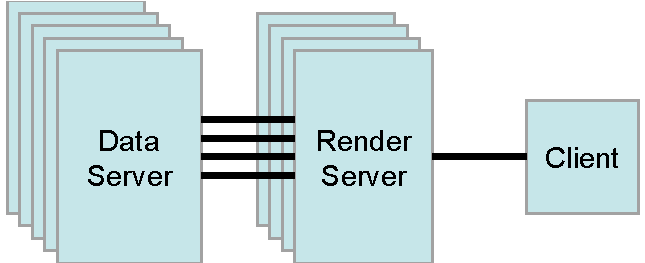
\includegraphics{images/RunModeClientRenderDataServer}
\end{inlinefig}

The third mode is \keyterm{client-render server-data server} mode.  In this
mode, all three logical units are running in separate programs.  As before,
the client is connected to the render server via a single socket
connection.  The render server and data server are connected by many socket
connections, one for each process in the render server.  Data transfer over
the sockets is minimized.

Although the client-render server-data server mode is supported, we almost
never recommend using it.  The original intention of this mode is to take
advantage of heterogeneous environments where one might have a large,
powerful computational platform and a second smaller parallel machine with
graphics hardware in it.  However, in practice we find any benefit is
almost always outstripped by the time it takes to move geometry from the
data server to the render server.  If the computational platform is much
bigger than the graphics cluster, then use software rendering on the large
computational platform.  If the two platforms are about the same size just
perform all the computation on the graphics cluster.

\section{Setting up a ParaView Server}

Setting up standalone ParaView is usually trivial.  You can download a
pre-compiled binary, install it on your computer, and go.  Setting up a
ParaView server, however, is intrinsically harder.  First, you will have to
compile the server yourself.  Because there are so many versions of MPI,
the library that makes parallel programming possible, and each version of
MPI may be altered to match the communication hardware of a parallel
computer, it is impossible to reliably provide binary files to match every
possible combination.

To compile ParaView on a parallel machine, you will need the following.

\begin{itemize}
\item CMake cross-platform build setup tool
  (\href{http://www.cmake.org}{www.cmake.org})
\item MPI
\item OpenGL (or use Mesa 3D \href{http://www.mesa3d.org}{www.mesa3d.org}
  if otherwise unavailable)
\item Qt 4.6 (optional)
\item Python (optional)
\end{itemize}

Compiling without one of the optional libraries means a feature will not be
available.  Compiling without Qt means that you will not have the GUI
application and compiling without Python means that you will not have
scripting available.

To compile ParaView, you first run CMake, which will allow you to set up
compilation parameters and point to libraries on your system.  This will
create the make files that you then use to build ParaView.  For more
details on building a ParaView server, see the ParaView Wiki.

{
  \footnotesize
  \href{http://www.paraview.org/Wiki/Setting_up_a_ParaView_Server#Compiling}{http://www.paraview.org/Wiki/Setting\_up\_a\_ParaView\_Server\#Compiling}
}

Running ParaView in parallel is also intrinsically more difficult than
running the standalone client.  It typically involves a number of steps
that change depending on the hardware you are running on: logging in to
remote computers, allocating parallel nodes, launching a parallel program,
establishing connections, and tunneling through firewalls.

Client-server connections are established through the \texttt{paraview}
client application.  You connect to servers and disconnect from servers
with the \connect and \disconnect buttons.  When ParaView starts, it
automatically connects to the builtin server.  It also connects to
builtin whenever it disconnects~\disconnect from a server.  We have already
seen examples of both.

When you hit the \connect button, ParaView presents you with a dialog box
containing a list of known servers you may connect to.  This list of
servers can be both site- and user-specific.

\begin{inlinefig}
  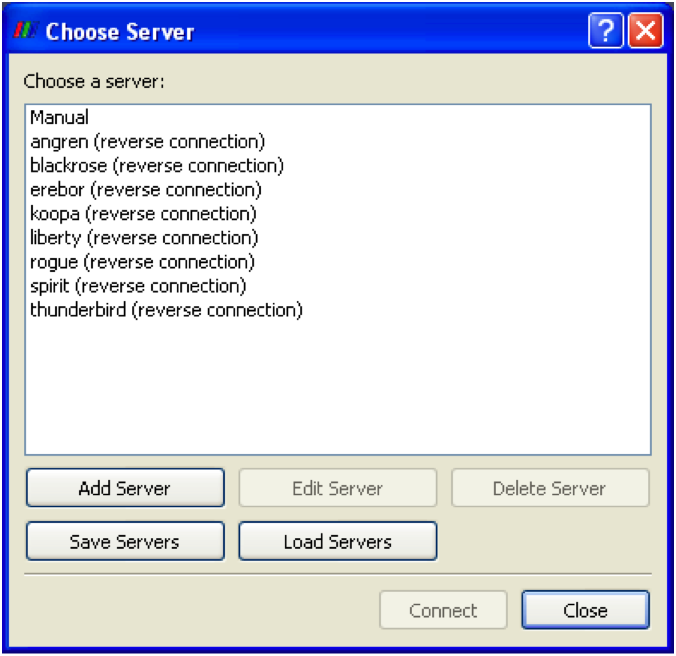
\includegraphics[width=2in]{images/ChooseServer}
\end{inlinefig}

You can specify how to connect to a server either through the GUI by
pressing the \gui{Add Server} button or through an XML definition file.
There are several options for specifying server connections, but ultimately
you are giving ParaView a command to run to launch the server and a host to
connect to after it is launched.  Consult the ParaView Wiki for more
information on establishing server connections.

{
  \footnotesize
  \href{http://www.paraview.org/Wiki/Setting_up_a_ParaView_Server#Running_the_Server}{http://www.paraview.org/Wiki/Setting\_up\_a\_ParaView\_Server\#Running\_the\_Server}
}


\section{Parallel Visualization Algorithms}

We are fortunate in that once you have a parallel framework, performing
parallel visualization tasks is straightforward.  The data we deal with is
contained in a mesh, which means the data is already broken into little
pieces by the cells.  We can do visualization on a distributed parallel
machine by first dividing the cells amongst the processes.  For
demonstrative purposes, consider this very simplified mesh.

\begin{inlinefig}
  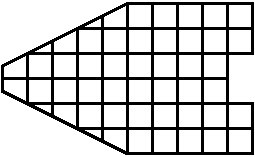
\includegraphics{images/ParallelExampleMesh}
\end{inlinefig}

Now let us say we want to perform visualizations on this mesh using three
processes.  We can divide the cells of the mesh as shown below with the
blue, yellow, and pink regions.

\begin{inlinefig}
  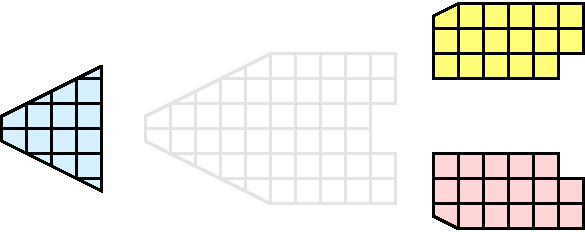
\includegraphics{images/ParallelExamplePartitions}
\end{inlinefig}

Once partitioned, some visualization algorithms will work by simply
allowing each process to independently run the algorithm on its local
collection of cells.  For example, take clipping.  Let us say that we
define a clipping plane and give that same plane to each of the processes.

\begin{inlinefig}
  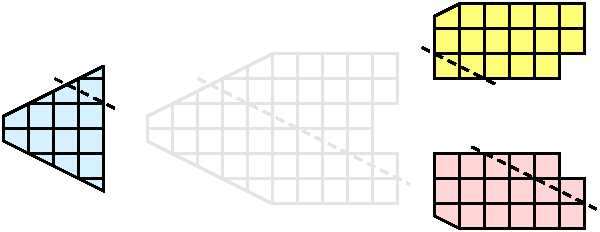
\includegraphics{images/ParallelExampleClip1}
\end{inlinefig}

Each process can independently clip its cells with this plane.  The end
result is the same as if we had done the clipping serially.  If we were to
bring the cells together (which we would never actually do for large data
for obvious reasons) we would see that the clipping operation took place
correctly.

\begin{inlinefig}
  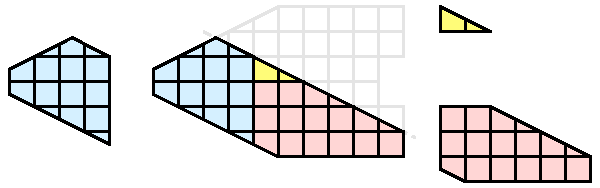
\includegraphics{images/ParallelExampleClip2}
\end{inlinefig}


\section{Ghost Levels}

Unfortunately, blindly running visualization algorithms on partitions of
cells does not always result in the correct answer.  As a simple example,
consider the \keyterm{external faces} algorithm.  The external faces
algorithm finds all cell faces that belong to only one cell, thereby
identifying the boundaries of the mesh.

\begin{inlinefig}
  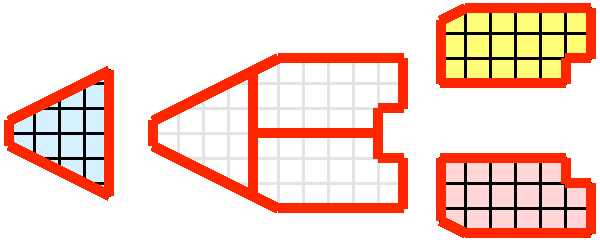
\includegraphics{images/ParallelExampleExternalFaces1}
\end{inlinefig}

Oops.  We see that when all the processes ran the external faces algorithm
independently, many internal faces where incorrectly identified as being
external.  This happens where a cell in one partition has a neighbor in
another partition.  A process has no access to cells in other partitions,
so there is no way of knowing that these neighboring cells exist.

The solution employed by ParaView and other parallel visualization systems
is to use \keyterm{ghost cells}.  Ghost cells are cells that are held in
one process but actually belong to another.  To use ghost cells, we first
have to identify all the neighboring cells in each partition.  We then copy
these neighboring cells to the partition and mark them as ghost cells, as
indicated with the gray colored cells in the following example.

\begin{inlinefig}
  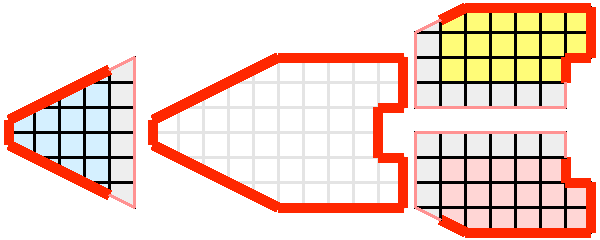
\includegraphics{images/ParallelExampleExternalFaces2}
\end{inlinefig}

When we run the external faces algorithm with the ghost cells, we see that
we are still incorrectly identifying some internal faces as external.
However, all of these misclassified faces are on ghost cells, and the faces
inherit the ghost status of the cell it came from.  ParaView then strips
off the ghost faces and we are left with the correct answer.

In this example we have shown one layer of ghost cells: only those cells
that are direct neighbors of the partition’s cells.  ParaView also has the
ability to retrieve multiple layers of ghost cells, where each layer
contains the neighbors of the previous layer not already contained in a
lower ghost layer or the original data itself.  This is useful when we have
cascading filters that each require their own layer of ghost cells.  They
each request an additional layer of ghost cells from upstream, and then
remove a layer from the data before sending it downstream.

\section{Data Partitioning}

Since we are breaking up and distributing our data, it is prudent to
address the ramifications of how we partition the data.  The data shown in
the previous example has a \keyterm{spatially coherent} partitioning.  That
is, all the cells of each partition are located in a compact region of
space.  There are other ways to partition data.  For example, you could
have a random partitioning.

\begin{inlinefig}
  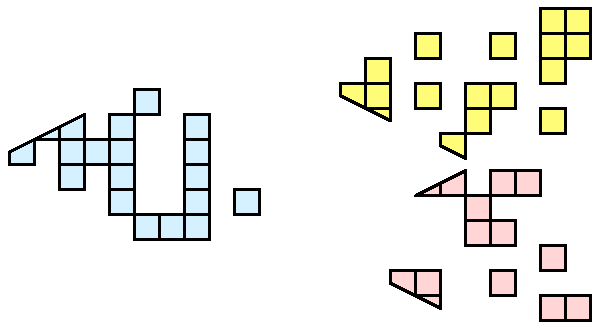
\includegraphics{images/ParallelExampleRandomPartition1}
\end{inlinefig}

Random partitioning has some nice features.  It is easy to create and is
friendly to load balancing.  However, a serious problem exists with respect
to ghost cells.

\begin{inlinefig}
  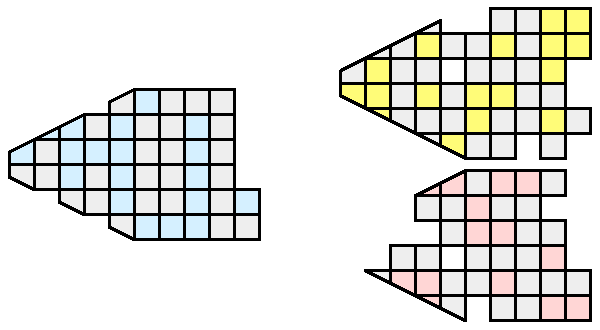
\includegraphics{images/ParallelExampleRandomPartition2}
\end{inlinefig}

In this example, we see that a single level of ghost cells nearly
replicates the entire data set on all processes.  We have thus removed any
advantage we had with parallel processing.  Because ghost cells are used so
frequently, random partitioning is not used in ParaView.

\section{D3 Filter}

The previous section described the importance of load balancing and ghost
levels for parallel visualization.  This section describes how to achieve
that.

Load balancing and ghost cells are handled automatically by ParaView when
you are reading structured data (image data, rectilinear grid, and
structured grid).  The implicit topology makes it easy to break the data
into spatially coherent chunks and identify where neighboring cells are
located.

It is an entirely different matter when you are reading in unstructured
data (poly data and unstructured grid).  There is no implicit topology and
no neighborhood information available.  ParaView is at the mercy of how the
data was written to disk.  Thus, when you read in unstructured data there
is no guarantee about how well load balanced your data will be.  It is also
unlikely that the data will have ghost cells available, which means that
the output of some filters may be incorrect.

Fortunately, ParaView has a filter that will both balance your unstructured
data and create ghost cells.  This filter is called D3, which is short for
distributed data decomposition.  Using D3 is easy; simply attach the filter
(located in \gui{Filters} \ra \gui{Alphabetical} \ra \gui{D3}) to whatever
data you wish to repartition.

\begin{inlinefig}
  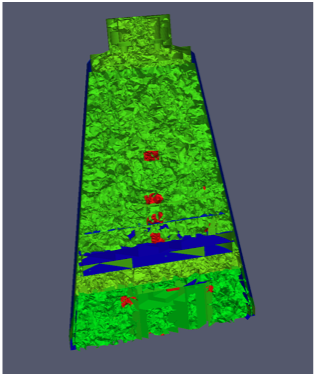
\includegraphics[height=1.65in]{images/D3ExampleBefore}
  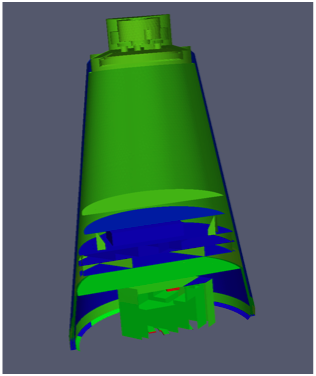
\includegraphics[height=1.65in]{images/D3ExampleAfter}
\end{inlinefig}

The most common use case for D3 is to attach it directly to your
unstructured grid reader.  Regardless of how well load balance the incoming
data might be, it is important to be able to retrieve ghost cell so that
subsequent filters will generate the correct data.  The example above shows
a cutaway of the extract surface filter on an unstructured grid.  On the
left we see that there are many faces improperly extracted because we are
missing ghost cells.  On the right the problem is fixed by first using the
D3 filter.


\section{Matching Job Size to Data Size}

\emph{How many processors should I have in my ParaView server?}  This is a
common question with many important ramifications.  It is also an
enormously difficult question.  The answer depends on a wide variety of
factors including what hardware each process has, how much data is being
processed, what type of data is being processed, what type of visualization
operations are being done, and your own patience.

Consequently, we have no hard answer.  We do however have several rules of thumb.

\textbf{If you are loading structured data} (image data, rectilinear grid,
structured grid), try to have a minimum of one processor per 20 million
cells.  If you can spare the processors, one processor for every 5 to 10
million cells is usually plenty.

\textbf{If you are loading unstructured data} (poly data, unstructured
grid), try to have a minimum of one processor per 1 million cells.  If you
can spare the processors, one processor for every 250 to 500 thousand cells
is usually plenty.

As stated before, these are just rules of thumb, not absolutes.  You should
always try to experiment to gage what your processor to data size should
be.  And, of course, there will always be times when the data you want to
load will stretch the limit of the resources you have available.  When this
happens, you will want to make sure that you avoid data explosion and that
you cull your data quickly.


\section{Avoiding Data Explosion}

The pipeline model that ParaView presents is very convenient for
exploratory visualization.  The loose coupling between components provides
a very flexible framework for building unique visualizations, and the
pipeline structure allows you to tweak parameters quickly and easily.

The downside of this coupling is that it can have a larger memory
footprint.  Each stage of this pipeline maintains its own copy of the data.
Whenever possible, ParaView performs \keyterm{shallow copies} of the data
so that different stages of the pipeline point to the same block of data in
memory.  However, any filter that creates new data or changes the values or
topology of the data must allocate new memory for the result.  If ParaView
is filtering a very large mesh, inappropriate use of filters can quickly
deplete all available memory.  Therefore, when visualizing large data sets,
it is important to understand the memory requirements of filters.

Please keep in mind that the following advice is intended \emph{only for
  when dealing with very large amounts of data and the remaining available
  memory is low}.  When you are not in danger of running out of memory,
ignore all of the following advice.

When dealing with structured data, it is absolutely important to know what
filters will change the data to unstructured.  Unstructured data has a much
higher memory footprint, per cell, than structured data because the
topology must be explicitly written out.  There are many filters in
ParaView that will change the topology in some way, and these filters will
write out the data as an unstructured grid, because that is the only data
set that will handle any type of topology that is generated.  The following
list of filters will write out a new unstructured topology in its output
that is roughly equivalent to the input.  These filters should \emph{never}
be used with structured data and should be used with caution on
unstructured data.

%TODO: there are surely more filters in each category now

\begin{multicols}{2}
  \begin{itemize}
  \item \gui{Append Datasets}
  \item \gui{Append Geometry}
  \item \gui{Clean}
  \item \gui{Clean to Grid}
  \item \gui{Connectivity}
  \item \gui{D3}
  \item \gui{Delaunay 2D/3D}
  \item \gui{Extract Edges}
  \item \gui{Linear Extrusion}
  \item \gui{Loop Subdivision}
  \item \gui{Reflect}
  \item \gui{Rotational Extrusion}
  \item \gui{Shrink}
  \item \gui{Smooth}
  \item \gui{Subdivide}
  \item \gui{Tessellate}
  \item \gui{Tetrahedralize}
  \item \gui{Triangle Strips}
  \item \gui{Triangulate}
  \end{itemize}
\end{multicols}

Technically, the \gui{Ribbon} and \gui{Tube} filters should fall into this
list.  However, as they only work on 1D cells in poly data, the input data
is usually small and of little concern.

This similar set of filters also output unstructured grids, but they also
tend to reduce some of this data.  Be aware though that this data reduction
is often smaller than the overhead of converting to unstructured data.
Also note that the reduction is often not well balanced.  It is possible
(often likely) that a single process may not lose any cells.  Thus, these
filters should be used with caution on unstructured data and extreme
caution on structured data.

\begin{multicols}{2}
  \begin{itemize}
  \item \gui{Clip}~\clip
  \item \gui{Decimate}
  \item \gui{Extract Cells by Region}
  \item \gui{Extract Selection}~\icon{pqExtractSelection24}
  \item \gui{Quadric Clustering}
  \item \gui{Threshold}~\threshold
  \end{itemize}
\end{multicols}

Similar to the items in the preceding list, \gui{Extract
  Subset}~\extractSubset performs data
reduction on a structured data set, but also outputs a structured data set.
So the warning about creating new data still applies, but you do not have
to worry about converting to an unstructured grid.

This next set of filters also outputs unstructured data, but it also
performs a reduction on the dimension of the data (for example 3D to 2D),
which results in a much smaller output.  Thus, these filters are usually
safe to use with unstructured data and require only mild caution with
structured data.

\begin{multicols}{2}
  \begin{itemize}
  \item \gui{Cell Centers}
  \item \gui{Contour}~\contour
  \item \gui{Extract CTH Fragments}
  \item \gui{Extract CTH Parts}
  \item \gui{Extract Surface}
  \item \gui{Feature Edges}
  \item \gui{Mask Points}
  \item \gui{Outline (curvilinear)}
  \item \gui{Slice}~\slice
  \item \gui{Stream Tracer}~\streamTracer
  \end{itemize}
\end{multicols}

These filters do not change the connectivity of the data at all.  Instead,
they only add field arrays to the data.  All the existing data is shallow
copied.  These filters are usually safe to use on all data.

\begin{multicols}{2}
  \begin{itemize}
  \item \gui{Block Scalars}
  \item \gui{Calculator}~\calculator
  \item \gui{Cell Data to Point Data}
  \item \gui{Curvature}
  \item \gui{Elevation}
  \item \gui{Generate Surface Normals}
  \item \gui{Gradient}
  \item \gui{Level Scalars}
  \item \gui{Median}
  \item \gui{Mesh Quality}
  \item \gui{Octree Depth Limit}
  \item \gui{Octree Depth Scalars}
  \item \gui{Point Data to Cell Data}
  \item \gui{Process Id Scalars}
  \item \gui{Random Vectors}
  \item \gui{Resample with dataset}
  \item \gui{Surface Flow}
  \item \gui{Surface Vectors}
  \item \gui{Texture Map to...}
  \item \gui{Transform}
  \item \gui{Warp (scalar)}
  \item \gui{Warp (vector)}~\warp
  \end{itemize}
\end{multicols}

This final set of filters are those that either add no data to the output
(all data of consequence is shallow copied) or the data they add is
generally independent of the size of the input.  These are almost always
safe to add under any circumstances (although they may take a lot of time).

\begin{multicols}{2}
  \begin{itemize}
  \item \gui{Annotate Time}
  \item \gui{Append Attributes}
  \item \gui{Extract Block}
  \item \gui{Extract Datasets}
  \item \gui{Extract Level}~\extractGroup
  \item \gui{Glyph}~\glyph
  \item \gui{Group Datasets}~\group
  \item \gui{Histogram}~\icon{pqHistogram24}
  \item \gui{Integrate Variables}
  \item \gui{Normal Glyphs}
  \item \gui{Outline}
  \item \gui{Outline Corners}
  \item \gui{Plot Global Variables Over Time}
  \item \gui{Plot Over Line}~\icon{pqPlotLineOverTime24}
  \item \gui{Plot Selection Over Time}~\icon{pqPlotCellOverTime24}
  \item \gui{Probe Location}~\icon{pqProbeLocation24}
  \item \gui{Temporal Shift Scale}
  \item \gui{Temporal Snap-to-Time-Steps}
  \item \gui{Temporal Statistics}
  \end{itemize}
\end{multicols}

There are a few special case filters that do not fit well into any of the
previous classes.  Some of the filters, currently \gui{Temporal
  Interpolator} and \gui{Particle Tracer}, perform calculations based on
how data changes over time.  Thus, these filters may need to load data for
two or more instances of time, which can double or more the amount of data
needed in memory.  The \gui{Temporal Cache} filter will also hold data for
multiple instances of time.  Also keep in mind that some of the temporal
filters such as the temporal statistics and the filters that plot over time
may need to iteratively load all data from disk.  Thus, it may take an
impractically long amount of time even if does not require any extra
memory.

The \gui{Programmable Filter}~\icon{pqProgrammableFilter24} is also a
special case that is impossible to classify.  Since this filter does
whatever it is programmed to do, it can fall into any one of these
categories.

\section{Culling Data}

When dealing with large data, it is clearly best to cull out data whenever
possible, and the earlier the better.  Most large data starts as 3D
geometry and the desired geometry is often a surface.  As surfaces usually
have a much smaller memory footprint than the volumes that they are derived
from, it is best to convert to a surface soon.  Once you do that, you can
apply other filters in relative safety.

A very common visualization operation is to extract isosurfaces from a
volume using the \gui{Contour}~\contour filter.  The \gui{Contour} filter
usually outputs geometry much smaller than its input.  Thus, the
\gui{Contour} filter should be applied early if it is to be used at all.
Be careful when setting up the parameters to the \gui{Contour} filter
because it still is possible for it to generate a lot of data.  This
obviously can happen if you specify many isosurface values.  High
frequencies such as noise around an isosurface value can also cause a
large, irregular surface to form.

Another way to peer inside of a volume is to perform a \gui{Slice}~\slice
on it.  The \gui{Slice}~\slice filter will intersect a volume with a plane
and allow you to see the data in the volume where the plane intersects.  If
you know the relative location of an interesting feature in your large data
set, slicing is a good way to view it.

If you have little \emph{a-priori} knowledge of your data and would like to
explore the data without paying the memory and processing time for the full
data set, you can use the \gui{Extract Subset}~\extractSubset filter to
subsample the data.  The subsampled data can be dramatically smaller than
the original data and should still be well load balanced.  Of course, be
aware that you may miss small features if the subsampling steps over them
and that once you find a feature you should go back and visualize it with
the full data set.

There are also several features that can pull out a subset of a volume:
\gui{Clip}~\clip, \gui{Threshold}~\threshold, \gui{Extract Selection}, and
\gui{Extract Subset}~\extractSubset can all extract cells based on some
criterion.  Be aware, however, that the extracted cells are almost never
well balanced; expect some processes to have no cells removed.  Also, all
of these filters with the exception of \gui{Extract Subset}~\extractSubset
will convert structured data types to unstructured grids.  Therefore, they
should not be used unless the extracted cells are of at least an order of
magnitude less than the source data.

When possible, replace the use of a filter that extracts 3D data with one
that will extract 2D surfaces.  For example, if you are interested in a
plane through the data, use the \gui{Slice}~\slice filter rather than the
\gui{Clip}~\clip filter.  If you are interested in knowing the location of
a region of cells containing a particular range of values, consider using
the \gui{Contour}~\contour filter to generate surfaces at the ends of the
range rather than extract all of the cells with the
\gui{Threshold}~\threshold filter.  Be aware that substituting filters can
have an effect on downstream filters.  For example, running the
\gui{Histogram}~\icon{pqHistogram24} filter after
\gui{Threshold}~\threshold will have an entirely different effect then
running it after the roughly equivalent \gui{Contour}~\contour filter.


\section{Rendering}

Rendering is the process of synthesizing the images that you see based on
your data.  The ability to effectively interact with your data depends
highly on the speed of the rendering.  Thanks to advances in 3D hardware
acceleration, fueled by the computer gaming market, we have the ability to
render 3D quickly even on moderately priced computers.  But, of course, the
speed of rendering is proportional to the amount of data being rendered.
As data gets bigger, the rendering process naturally gets slower.

To ensure that your visualization session remains interactive, ParaView
supports two modes of rendering that are automatically flipped as
necessary.  In the first mode, \keyterm{still render}, the data is rendered
at the highest level of detail.  This rendering mode ensures that all of
the data is represented accurately.  In the second mode,
\keyterm{interactive render}, speed takes precedence over accuracy.  This
rendering mode endeavors to provide a quick rendering rate regardless of
data size.

While you are interacting with a 3D view, for example rotating, panning, or
zooming with the mouse, ParaView uses an interactive render.  This is
because during the interaction a high frame rate is necessary to make these
features usable and because each frame is immediately replaced with a new
rendering while the interaction is occurring so that fine details are less
important during this mode.  At any time when interaction of the 3D view is
not taking place, ParaView uses a still render so that the full detail of
the data is available as you study it.  As you drag your mouse in a 3D view
to move the data, you may see an approximate rendering while you are moving
the mouse, but the full detail will be presented as soon as you release the
mouse button.

The interactive render is a compromise between speed and accuracy.  As
such, many of the rendering parameters concern when and how lower levels of
detail are used.

\subsection{Basic Parameter Settings}

Some of the most important rendering options are the LOD parameters.
During interactive rendering, the geometry may be replaced with a lower
\keyterm{level of detail} (\keyterm{LOD}), an approximate geometry with
fewer polygons.

\begin{inlinefig}
  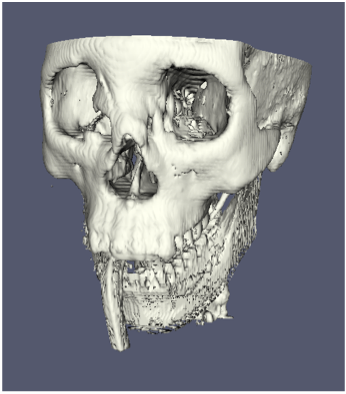
\includegraphics[width=1.5in]{images/GeometricLODFull}
  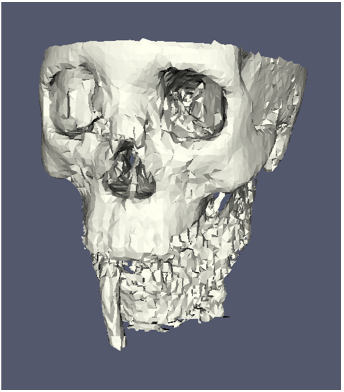
\includegraphics[width=1.5in]{images/GeometricLOD50}
  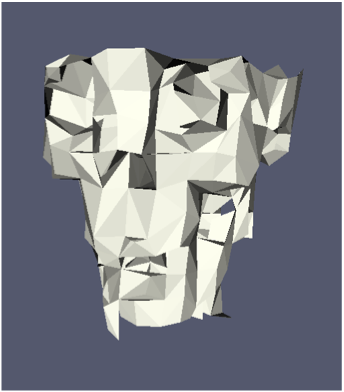
\includegraphics[width=1.5in]{images/GeometricLOD10}
\end{inlinefig}

The resolution of the geometric approximation can be controlled.  The
decimation algorithm strives to place the polygons in a coarse grid.  In
the proceeding images, the left image is the full resolution; the middle
image is decimation on a $50^3$ grid, and the right image is decimation on
a $10^3$ grid.

The 3D rendering parameters are located in the settings dialog box which is
accessed in the menu from \gui{Edit} \ra \gui{Settings} (\gui{ParaView} \ra
\gui{Preferences} on the Mac).  The basic rendering options in the dialog
are in the \gui{Render View} \ra \gui{General} section.

\begin{inlinefig}
  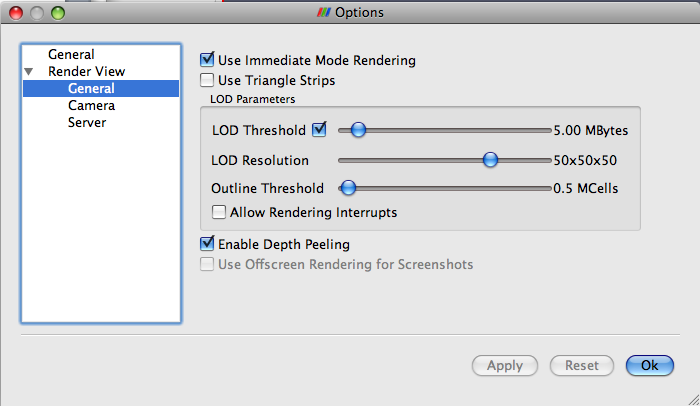
\includegraphics[width=3in]{images/SettingsRendering}
\end{inlinefig}

The options pertaining to rendering performance have the following
meanings.

\begin{description}
\item[Use Immediate Mode Rendering] \index{immediate mode rendering} When
  checked, geometry is sent to the graphics card for immediate rendering.
  When unchecked, the geometry is first compiled into display lists for
  more efficient rendering.  The display lists usually render faster, but
  require initial time to compile during the first frame and extra memory
  to store.
\item[Use Triangle Strips] \index{triangle strips} When unchecked, data is
  rendered as defined in the poly data.  When checked, the data is first
  converted to triangle strips.  Triangle strips can be pushed to a
  graphics card more efficiently and can sometimes be rendered faster, but
  not usually.
\item[LOD Threshold] \index{LOD Threshold}Controls when to replace the
  geometry with a decimated version of the geometry.  The checkbox turns
  the feature on or off.  When on, the slider gives a threshold for the
  feature.  If the geometry size is below the threshold, it is considered
  small enough to render.  When the geometry size is above the threshold,
  the decimated form is used during rendering.
\item[Allow Rendering Interrupts] \index{rendering interrupts} When
  checked, a still render may be interrupted by a request to perform an
  interactive render.
\end{description}

\subsection{Basic Parallel Rendering}

When performing parallel visualization, we are careful to ensure that the
data remains partitioned amongst all of the processes up to and including
the rendering processes.  ParaView uses a parallel rendering library called
\keyterm{IceT}.  IceT uses a \keyterm{sort-last} algorithm for parallel
rendering.  This parallel rendering algorithm allows each process to
independently render its partition of the geometry and then
\keyterm{composites} the partial images together to form the final image.

\begin{inlinefig}
  \includegraphics{images/ParallelRendering}
\end{inlinefig}

The preceding diagram is an oversimplification.  IceT contains multiple
parallel image compositing algorithms such as \keyterm{binary tree} and
\keyterm{binary swap} that efficiently divide work amongst processes using
multiple phases.

\begin{inlinefig}
  \includegraphics{images/ParallelRenderingDetail}
\end{inlinefig}

The wonderful thing about sort-last parallel rendering is that its
efficiency is completely insensitive to the amount of data being rendered.
This makes it a very scalable algorithm and well suited to large data.
However, the parallel rendering overhead does increase linearly with the
number of pixels in the image.  Consequently, some of the rendering
parameters deal with the image size.

\begin{inlinefig}
  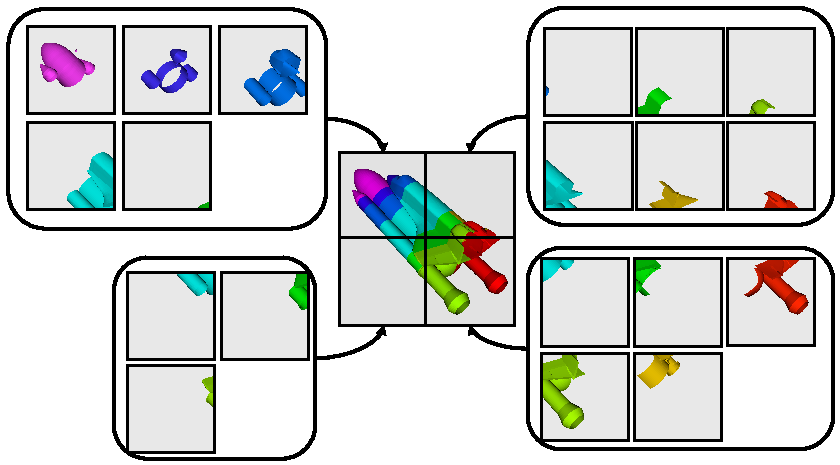
\includegraphics{images/ParallelRenderingTiles}
\end{inlinefig}

IceT also has the ability to drive tiled displays, large, high-resolution
displays comprising an array of monitors or projectors.  Using a sort-last
algorithm on a tiled display is a bit counterintuitive because the number
of pixels to composite is so large.  However, IceT is designed to take
advantage of spatial locality in the data on each process to drastically
reduce the amount of compositing necessary.  This spatial locality can be
enforced by applying the \gui{D3} filter to your data.

Because there is an overhead associated with parallel rendering, ParaView
has the ability to turn off parallel rendering at any time.  When parallel
rendering is turned off, the geometry is shipped to the location where
display occurs.  Obviously, this should only happen when the data being
rendered is small.

\subsection{Parallel Render Parameters}

\begin{inlinefig}
  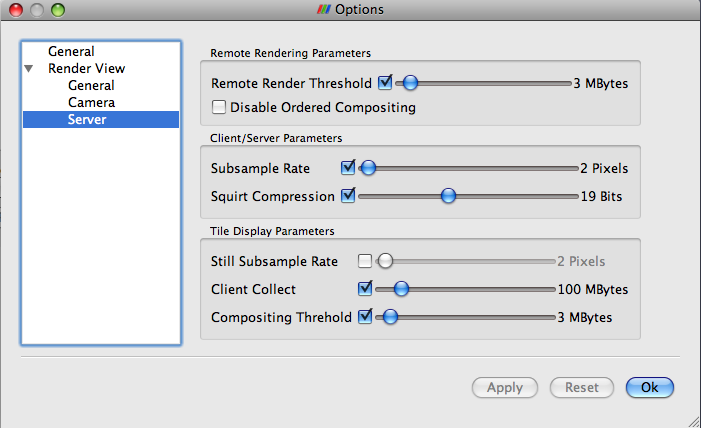
\includegraphics[width=3in]{images/SettingsServer}
\end{inlinefig}

Like the other 3D rendering parameters, the parallel rendering parameters
are located in the settings dialog box which is accessed in the menu from
\gui{Edit} \ra \gui{Settings} (\gui{ParaView} \ra \gui{Preferences} on the
Mac).  The parallel rendering options in the dialog are in the \gui{Render
  View} \ra \gui{Server} section.  The options have the following meanings.

\begin{description}
\item[Remote Render Threshold] \index{remote render threshold} The checkbox
  turns remote rendering on or off.  The slider controls the threshold at
  which to use parallel rendering.  Whenever the geometry is below the
  threshold, the geometry is moved to the location where display occurs
  (usually the client).
\item[Suppress Ordered Compositing] \index{ordered compositing} To view
  volume rendering and transparent polygons correctly, a special parallel
  rendering mode called ordered compositing is required.  However, this
  mode has some additional computation and memory.  Checking this box
  prevents ordered compositing from ever happening.
\item[Interactive Subsample Rate] \index{subsample} The overhead of parallel rendering
  is proportional to the size of the images generated.  Thus, you can speed
  up interactive rendering by specifying an image subsampling rate.  When
  this box is checked, interactive renders will create smaller images,
  which are then magnified when displayed.  This parameter is only used
  during interactive renders.  A full resolution image is always used
  during a still render.
\item[Image Compression] Before images are shipped from server to client,
  they can be compressed using one of two compression algorithms.
  \keyterm{SQUIRT} or \keyterm{Zlib}. To make the compression
  more effective, either algorithm can reduce the color resolution of
  the image before compression.  The sliders determine the amount of color
  bits saved.  Full color resolution is always used during a still render.
\item[Still Subsample Rate] Tiled displays are often used for multiple
  things.  For example, the display may be used for small collaborations or
  during large presentations.  In the large presentation, the audience is
  unlikely to be able to resolve all of the pixels in the display.  If that
  is the case, this option allows you to subsample the still renders and
  save a significant amount of time.
\item[Client Collect] \index{client collect} When in tiled display mode,
  the parallel rendering is sent to the tiled display, not the desktop.
  Thus, the client must render all of its data locally.  This parameter
  sets a limit on the amount of data sent to the client.  If the data is
  larger than the set threshold, the client will simply show a bounding box
  around the data.
\item[Compositing Threshold] \index{compositing threshold} The compositing
  threshold is the equivalent of the remote render threshold for tiled
  displays.  The trade offs for performing compositing are different.
  Tiled displays typically have a higher overhead for compositing due to
  their higher resolution displays and they have a lower overhead for
  geometry collection because it is usually done within a high speed
  network.  Thus, it might make sense to set the compositing threshold
  higher than the remote render threshold.  If the geometry size is under
  the compositing threshold, then the entire visible geometry will be
  broadcast to all rendering nodes and each will render directly to their
  tile.
\end{description}

\subsection{Parameters for Large Data}

The default rendering parameters are suitable for most users.  However,
when dealing with very large data, it can help to tweak the rendering
parameters.  The optimal parameters depend on your data and the hardware
ParaView is running on, but here are several pieces of advice that you
should follow.

\begin{enumerate}
\item Turn \gui{Use Immediate Mode Rendering} on and turn \gui{Use Triangle
  Strips} off.  Both of these options are intending to convert your data
  into structures that are more efficiently rendered.  However, the
  processing and memory overhead are often not worth it when data is large.
  In fact, when the memory limits are stretched, this can actually reduce
  performance.
\item Try turning the \gui{LOD Threshold} \emph{off}.  The geometry
  decimation can take a long time with large data, and it sometimes does a
  poor job if your data has high curvatures or strange connectivity.  If
  the LOD is improving your performance, try moving the \gui{LOD
    Resolution} slider all the way to the right (10x10x10).
\item Always have remote rendering on (controlled by the checkbox next to
  \gui{Remote Render Threshold}).  The remote rendering will use the power
  of entire server to render and ship images to the client.  If remote
  rendering is off, geometry is shipped back to the client.  When you have
  large data, it is always faster to ship images than to ship data.
\item Turn on subsampling and adjust the \gui{Subsample Rate} as needed.
  If image compositing is slow, if the connection between client and server
  has low bandwidth, or if you are rendering very large images, then a
  higher subsample rate can greatly improve your interactive rendering
  performance.
\item Make sure \gui{Image Compression} is on.  It has a tremendous effect
  on desktop delivery performance, and the artifacts it introduces, which
  are only there during interactive rendering, are minimal.
\end{enumerate}


% Chapter Visualizing Large Models
